\chapter{Plasma Overview}
\label{ch:plasma_overview}

Plasma is a fundamental state of matter, along with solid, liquid, and gas. It has similar characteristics to gases, where it is compressible and does not conform to a specific shape; however the key difference is that plasmas are highly electrically conductive, even capable of producing their own magnetic field. This is because plasmas contain a large number of positive ions that interact in a `sea' of free-moving electrons.

\section{Plasma Discharge}

Plasmas are generated in one of two primary ways. The first is via extreme heating of a gas whereby the electrons gain sufficient energy to escape the electromagnetic force of the nucleus. The most obvious example of this is in stars where the gases within reach temperatures millions of degrees Kelvin, giving rise to nuclear fusion. The other method, which is the main focus of this report, is the exposure of a gas to a large electric field. This in turn ignites the plasma in a process described in the rest of this chapter. An everyday example of this is lightning, where charges build up between the clouds and the ground, which in turn causes the potential difference between the two to grow until the air in between breaks down.

\subsection{Paschen's Law}
\label{sec:paschens_law}

The voltage necessary to break down a gas is given by Paschen's law. It states that the breakdown voltage is a function of two parameters \cite{Lieberman2005}: the pressure of the gas and the distance between the electrodes (referred to as the gap length). Specifically, the breakdown voltage is given by the product of these two parameters.

In order for breakdown to occur, there needs to be a small number of electrons already present in the gas. This can be caused internally by a smaller number of already excited gas molecules, or externally by highly energetic cosmic rays entering the gas chamber. Then by applying a voltage, these electrons gain energy creating other electrons via ionising collisions. When more electrons are generated from the collisions than are lost, an avalanche is created, which causes the gas breakdown.

The breakdown voltage can be expressed by the following equation \cite{Lieberman2005}:

\begin{equation}
	V_B = \frac{B p d}{ln(A p d) - ln[ln(1-\frac{1}{\gamma_{se}})]}
\end{equation}

where $V_B$ is the breakdown voltage, $p$ is the pressure of the gas, $d$ is the gap length, $\gamma_{se}$ is the coefficient for secondary-electron emission (explained in section 2.1.2), and $A$ and $B$ are constants for a given gas that are determined experimentally.

However it is much easier to understand Paschen's law pictorially. Figure \ref{fig:pashen_curve} illustrates the voltage breakdown curves for various gases. Each curve is slightly different, however all of them do exhibit a convex shape. Supposing if:

\begin{itemize}
    \item \textbf{The gap length remains constant}. Starting with a large pressure, the mean free path of an electron within the gas is quite short, meaning it does not have sufficient time in between collisions for it to gain enough energy to cause an ionising collision with the neutral gas. As the pressure is then reduced, the mean free path increases, making it easier for the electrons to gain sufficient energy to undergo ionising collisions; until a certain critical pressure that is (typically a $pd$ of approximately 1 to 10 Torr cm). Beyond this, decreasing the pressure further causes the mean free path of the electron lengthen to a point that is comparable to the gap length, therefore this decreases the likelihood of an electron colliding with a neutral gas particle and the breakdown voltage increases.
    \item \textbf{The pressure remains constant}. When the gap length is very small, electrons are accelerated by a large electric field but are collected by the electrodes without undergoing collisions with the background gas. Increasing this gap length to a certain point gives the electrons the opportunity to collide with the background gas, producing ionising collisions. However, as the gap length continues to be increased, the strength of the electric field between the electrodes decreases, hence the electrons gain less energy between the collisions resulting in fewer ionising collisions with the background gas.
\end{itemize}

\begin{figure}[h!]
	\centering
	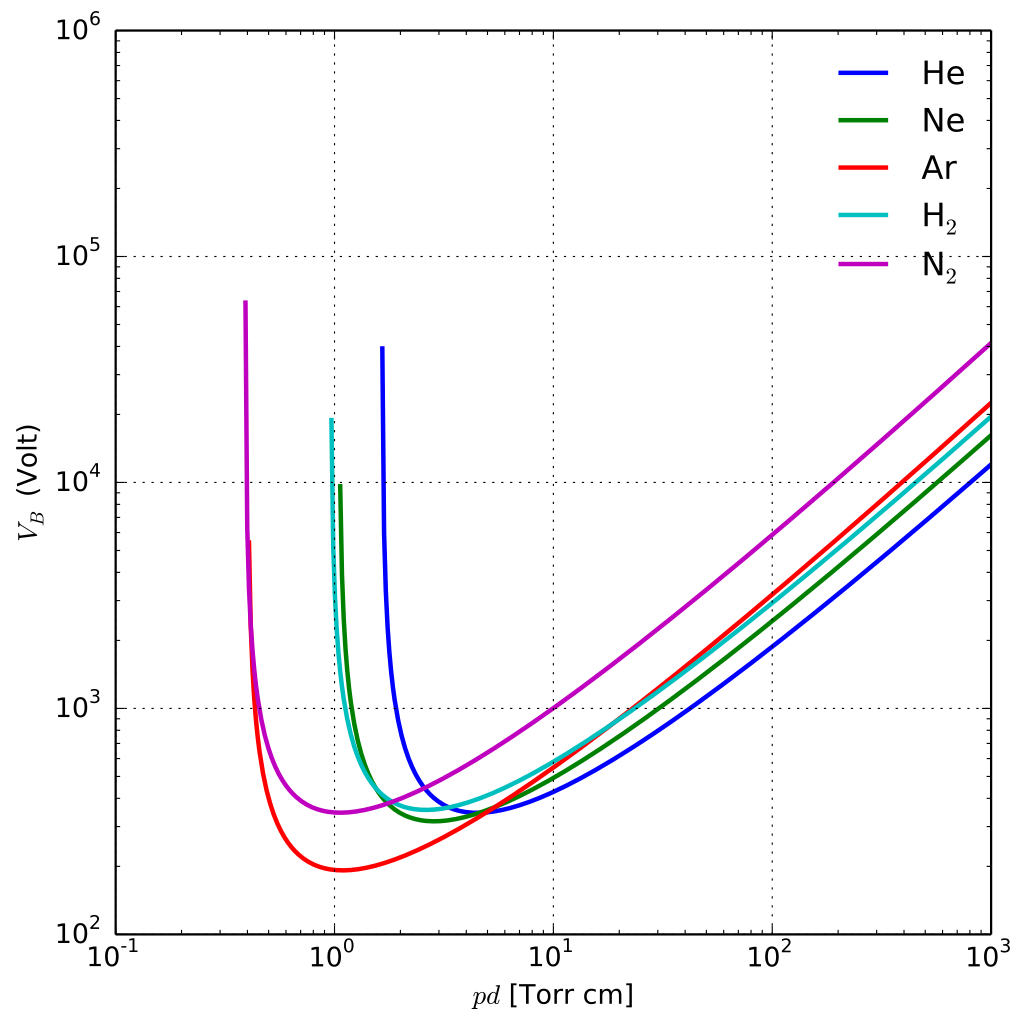
\includegraphics[width=0.6\linewidth]{chapter_2/figures/paschen_curve.png}
	\caption{Paschen curve for Helium, Neon, Argon, Hydrogen, and Nitrogen gases \cite{Lieberman2005}.}
	\label{fig:pashen_curve}
\end{figure}

\subsection{DC Discharge}

Consider a circuit as seen in figure \ref{fig:basic_circuit}. Two parallel electrodes with a DC voltage applied, and a neutral gas contained within a chamber. As the resistance of the variable resistor is decreased, which in turn increases the current through the plasma, one would observe three distinct discharge regions \cite{Gudmundsson2017}, observed in figure \ref{fig:dc_discharge}.

\begin{figure}[h!]
	\centering
	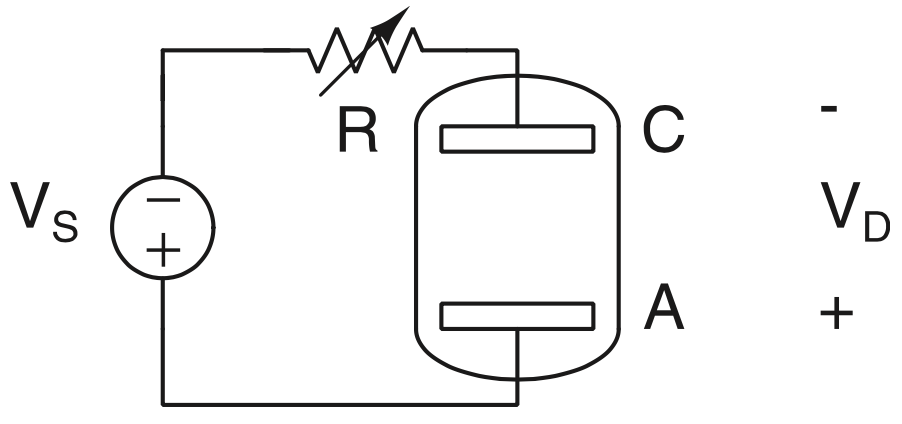
\includegraphics[width=0.6\linewidth]{chapter_2/figures/basic_circuit.png}
	\caption{Circuit diagram with a source voltage ($V_s$) and variable resistor ($R$) to control the current through a discharge region ($C$ to $A$) \cite{Gudmundsson2017}.}
	\label{fig:basic_circuit}
\end{figure}

The first, is the dark discharge (or sometime referred to as the Townsend discharge) region. Initially, the voltage between the electrodes builds up as the only current through the plasma is caused by pre-existing electrons, say from cosmic radiation; however this current quickly saturates (seen from region A-B in figure \ref{fig:dc_discharge}). Then, once the electrons gain sufficient energy, they begin colliding with the background gas to produce additional electrons in a process called the \textit{Townsend avalanche} (seen from region B-D in figure \ref{fig:dc_discharge}). Once this avalanche is self-sustaining, the voltage breakdown of the gas is reached (at point D in figure \ref{fig:dc_discharge}).

\begin{figure}[h!]
	\centering
	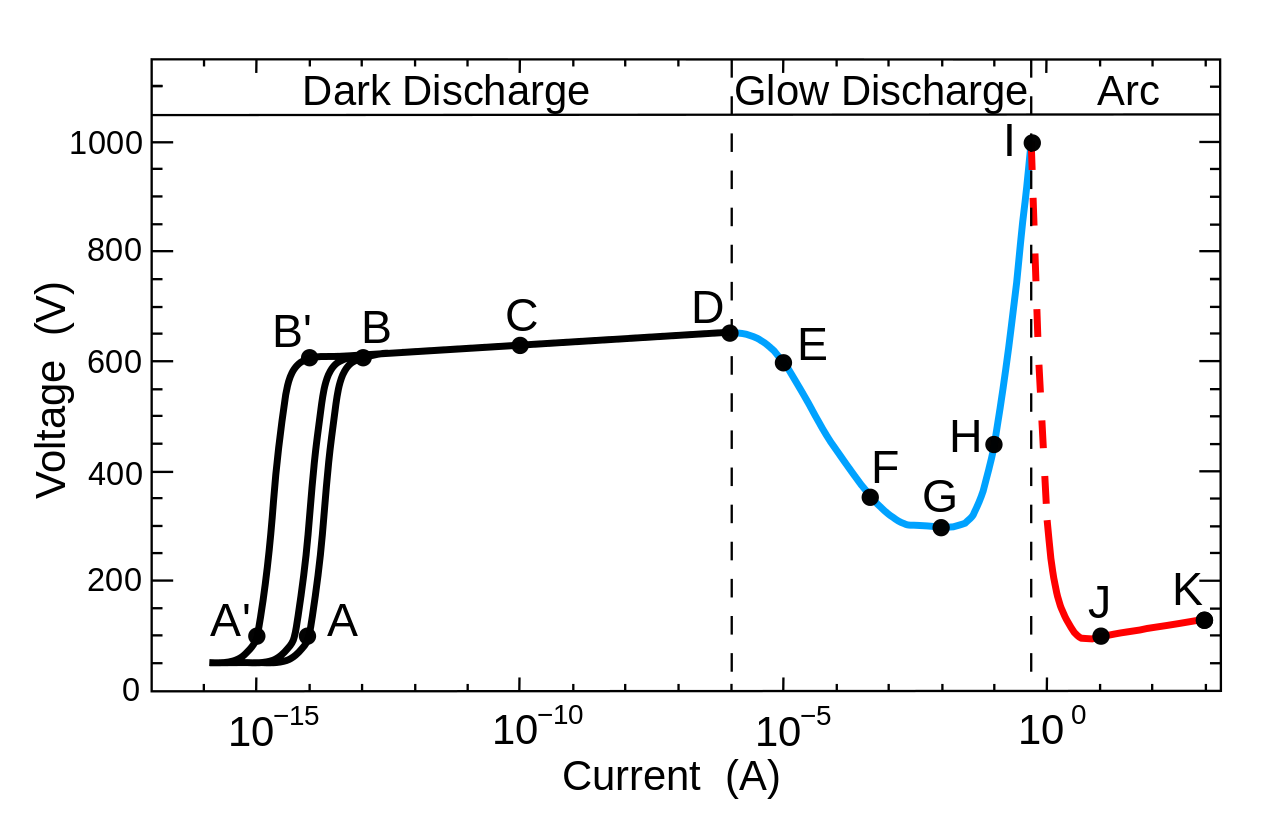
\includegraphics[width=0.8\linewidth]{chapter_2/figures/dc_discharge.png}
	\caption{Depiction of the current-voltage relationship across three discharge regions \cite{Gallo1975}.}
	\label{fig:dc_discharge}
\end{figure}

After the breakdown, the plasma is said to be in a glow discharge region. Here, the voltage across the plasma decreases since a transition from a gas to plasma state causes a decrease in resistance, implying that the ionisation process from the avalanche is more efficient (seen from region D-G in figure \ref{fig:dc_discharge}). This efficiency stems from the fact that the electrons are generated by a secondary means in addition to the standard Townsend avalanche. This process is called the secondary emission of electrons, which is caused the energetic collisions of ions and metastables with the surface of the cathode. These \textit{secondary-electrons} are then accelerated by the electric field and cause further Townsend avalanches.

At first, ion bombardment on the surface of the cathode is non-uniform but as the current generated from this increases, it eventually stabilises and the distribution of the plasma (and thus the ions) across the cathode become more uniform. This is referred to as \textit{subnormal glow} and \textit{normal glow} respectively. As the current is increased further, ion bombardment across the cathode becomes saturated as it covers the entire surface of the cathode (seen from region G-I in figure \ref{fig:dc_discharge}). This is referred to as \textit{abnormal glow}, and increasing the current further causes the glow discharge to become an arc (at point I in figure \ref{fig:dc_discharge}).

In the arc discharge region, the ion bombardment onto the cathode causes the cathode to heat up to a point where electrons are generated via thermionic emission. This significantly reduces the resistance of the plasma, causing a very large drop of the voltage (seen from region I-J in figure \ref{fig:dc_discharge}). 

For the purposes of this project, the arc discharge region will be avoided. The reason being, operating under arc conditions increases the electrode sputtering rate. \textit{Sputtering} is the ejection of atoms from the electrode caused by the bombardment of energetic particles. While useful for processes such as ion etching \cite{Lieberman2005}, sputtering would not be favourable for the as the consumption of the electrode material is something to be avoided. Sputtering has the additional downside of potentially contaminating the plasma composition as ejected atoms could end up reacting with the other plasma species. 

\begin{figure}[h!]
	\centering
	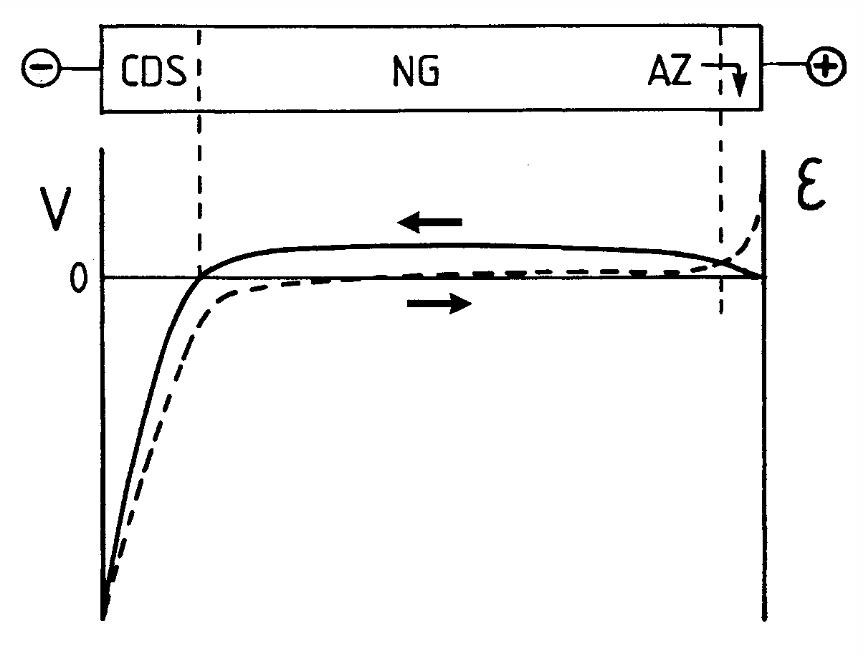
\includegraphics[width=0.7\linewidth]{chapter_2/figures/glow_discharge.png}
	\caption{Schematic highlighting the regions present in a DC glow discharge \cite{Bogaerts2002}. The cathode is on the left and the grounded anode is on the right. (CDS is the cathode dark space, NG is the negative glow, and AZ is the anode dark space.}
	\label{fig:glow_discharge}
\end{figure}

In a glow discharge there are typical three spatial regions present. These include a \textit{cathode dark space}, a \textit{negative glow} region, and the \textit{anode dark space} \cite{Gudmundsson2017, Bogaerts2002}. This can be observed in figure \ref{fig:glow_discharge}, that shows the potential in each region. Do note, as the distance between the electrodes is increased, additional regions may develop, however these three regions will always persist. The dark space regions are called \textit{sheaths} while the negative glow region is known as the \textit{bulk plasma}. Generally, the sheaths on the cathode will be much larger than that of the anode, as it corresponds to the region where electrons are being accelerated before gaining sufficient energy to cause ionising collisions. In contrast, the anode sheaths form to limit the electron current to the anode, maintaining current continuity over the discharge. Finally, the bulk plasma is the quasi-neutral region that contains the ions and electrons of the plasma.

\subsection{AC Discharge}

If the voltage source in the circuit of figure \ref{fig:basic_circuit} were to be replaced with a low frequency AC source, the discharge behaviour would be almost identical to that of the DC discharge, with the caveat that the roles of the electrodes alternating between cathode and anode. This is provided that the half time period of an AC cycle is larger than the duration for ions and electrons to move across the electrodes \cite{Bogaerts2002}.

However, as the frequency of the AC source is increased, typically to the region of radio or microwave frequencies, there is an asymmetry between the movement of the ions and electrons. The electrons are capable of responding to the change in the electric fields relatively quickly; however, due to the ions being significantly heavier than electrons, they have a much slower response time that is restricted by their inertia \cite{Chabert2011}.

Since the ions cannot respond to the changing electric field quick enough, they respond to the time-averaged field thus are accelerated against both electrodes cross the sheath. On the other hand, the electrons begin accelerating through the bulk plasma towards the anode during the first half period of the AC signal. Then as the direction of the electric field reverses in the second half period of the signal, the positions of the anode and cathode flip, and any electron that has not collided with the original anode (which is now the cathode), gets accelerated through the bulk plasma towards the new anode. This oscillating behaviour confines the electrons, resulting in an increased likelihood of ionising collisions with the neutral background gas. As the frequency of the AC source is increased, more electrons become trapped in this regime, hence it is no surprise that the breakdown voltage of the plasma decreases \cite{Chu1992}. This can be seen in figure \ref{fig:ac_breakdown}

Astute readers may notice the minimal role of the secondary emission of electrons plays in the AC discharge. Because of the reduced of ion bombardments, there is less erosion on the electrodes, which increases its overall lifetime. 

\begin{figure}[h!]
	\centering
	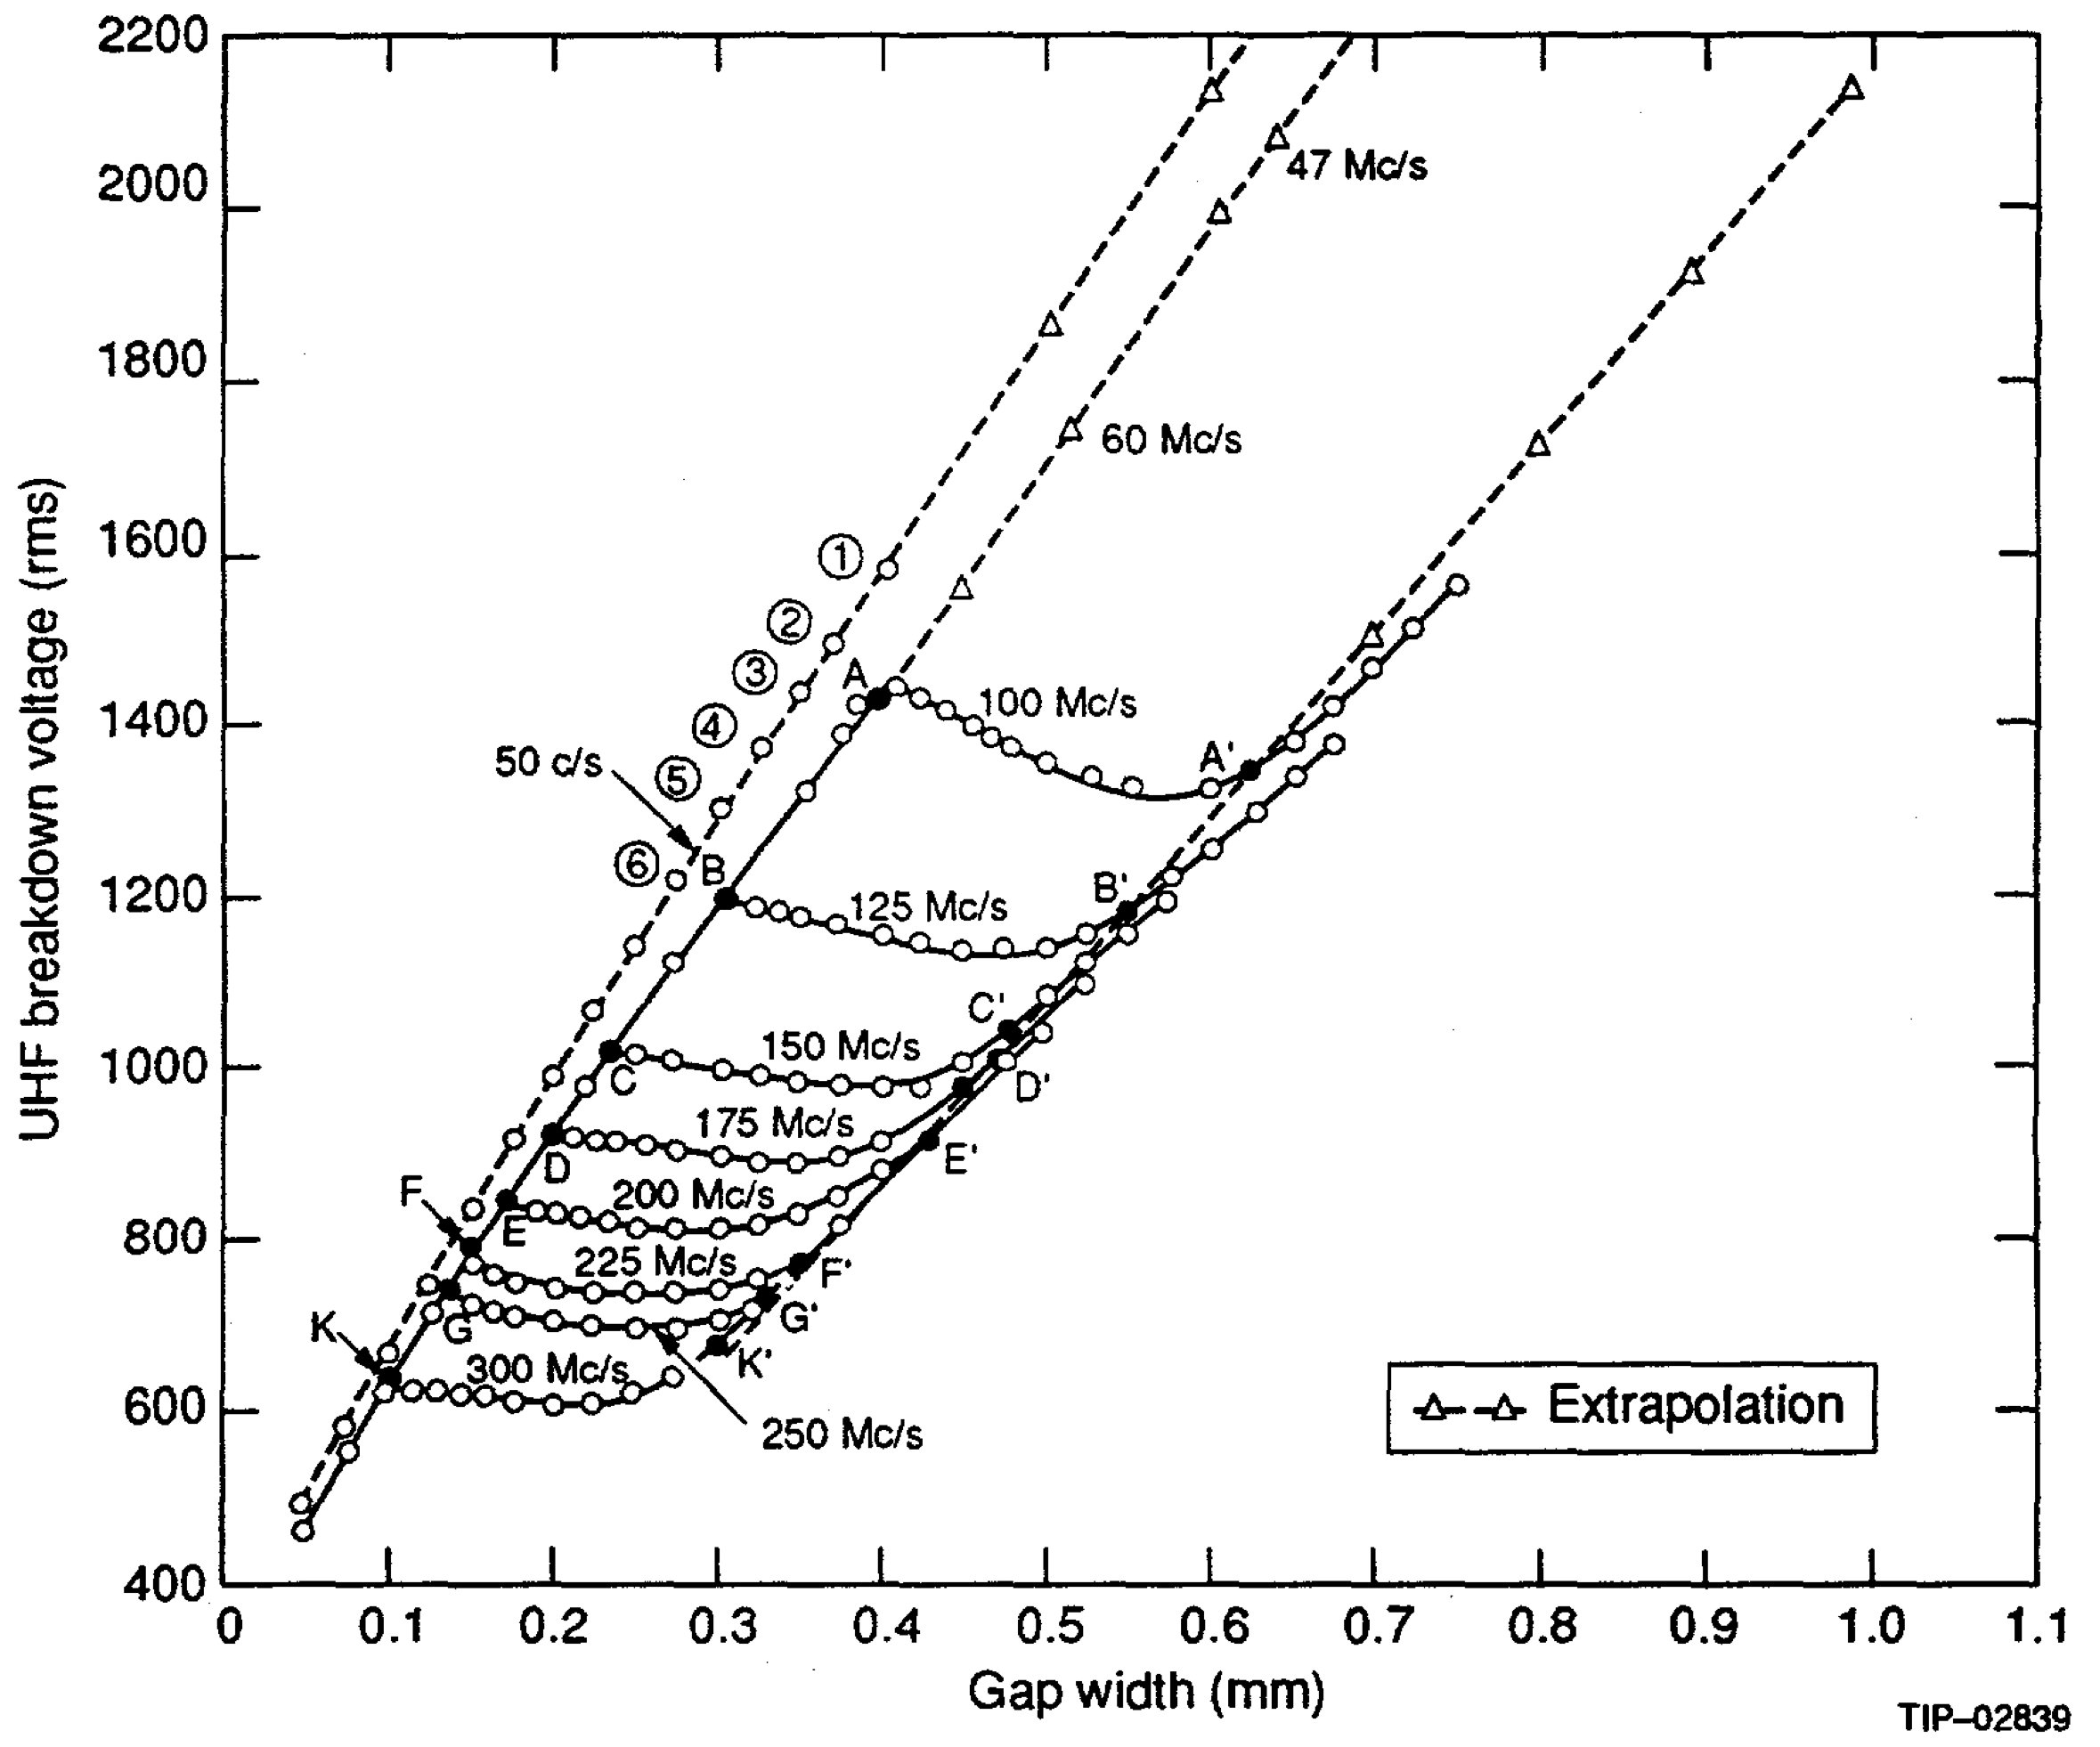
\includegraphics[width=\linewidth]{chapter_2/figures/ac_breakdown.png}
	\caption{Paschen curve for AC discharge across various frequencies \cite{Pim1949}.}
	\label{fig:ac_breakdown}
\end{figure} 


